\subsection{Geräteübersicht}
\label{shap:Geraeteuebersicht}
Der Ballwerfer ist so konzipiert, das er aus einem fix stehenden Basismodul besteht, 
welches in der Mitte des Startbereiches positioniert wird. Die Abwurfeinheit, 
welche den Ballwurfmechanismus und die Ballzuführung beinhaltet, ist auf dem 
Basismodul drehend gelagert. Ein Motor richtet die Abwurfeinheit auf das Ziel aus. 
Der ganze Aufbau des Ballwurfmechanismus ist möglichst einfach gehalten. Er besteht 
hauptsächlich aus zwei Acrylglasplatten, in welcher alle mechanischen Vorrichtungen 
gelagert sind.  Dadurch kann der ganze Aufbau schnell und einfach angepasst oder 
geändert werden. Die Ausrichtung des Abwurfmechanismus erfolgt durch einen Motor, 
welcher in der drehenden Abwurfeinheit angebracht ist. Dadurch kann die Bauhöhe 
des Ballwerfers tief gehalten werden, was einen grossen Stabilitätsvorteil bietet. 
Die Drehachse der Abwurfeinheit ist an der Spitze des Ballwerfers mit einem Bolzen 
angebracht. Somit bleibt die Abwurfposition der Tennisbälle konstant am gleichen Ort.\\
\\
Die Tennisbälle werden durch zwei Schwungräder beschleunigt. Die Schwungräder 
drehen gegenläufig, der Tennisball wird dazwischen ausgestossen. Die Zuführung der 
Tennisbälle erfolgt mit einem eigens gesteuerten Förderband. Das Förderband muss 
die Bälle mit konstanter Geschwindigkeit zu den Schwungrädern transportieren, damit 
alle Tennisbälle die gleiche Startenergie aufweisen. Dadurch ist eine gleichmässige
 Wurfweite und eine hohe Reproduzierbarkeit gewährleistet.
\begin{figure}[h!]
		\centering
		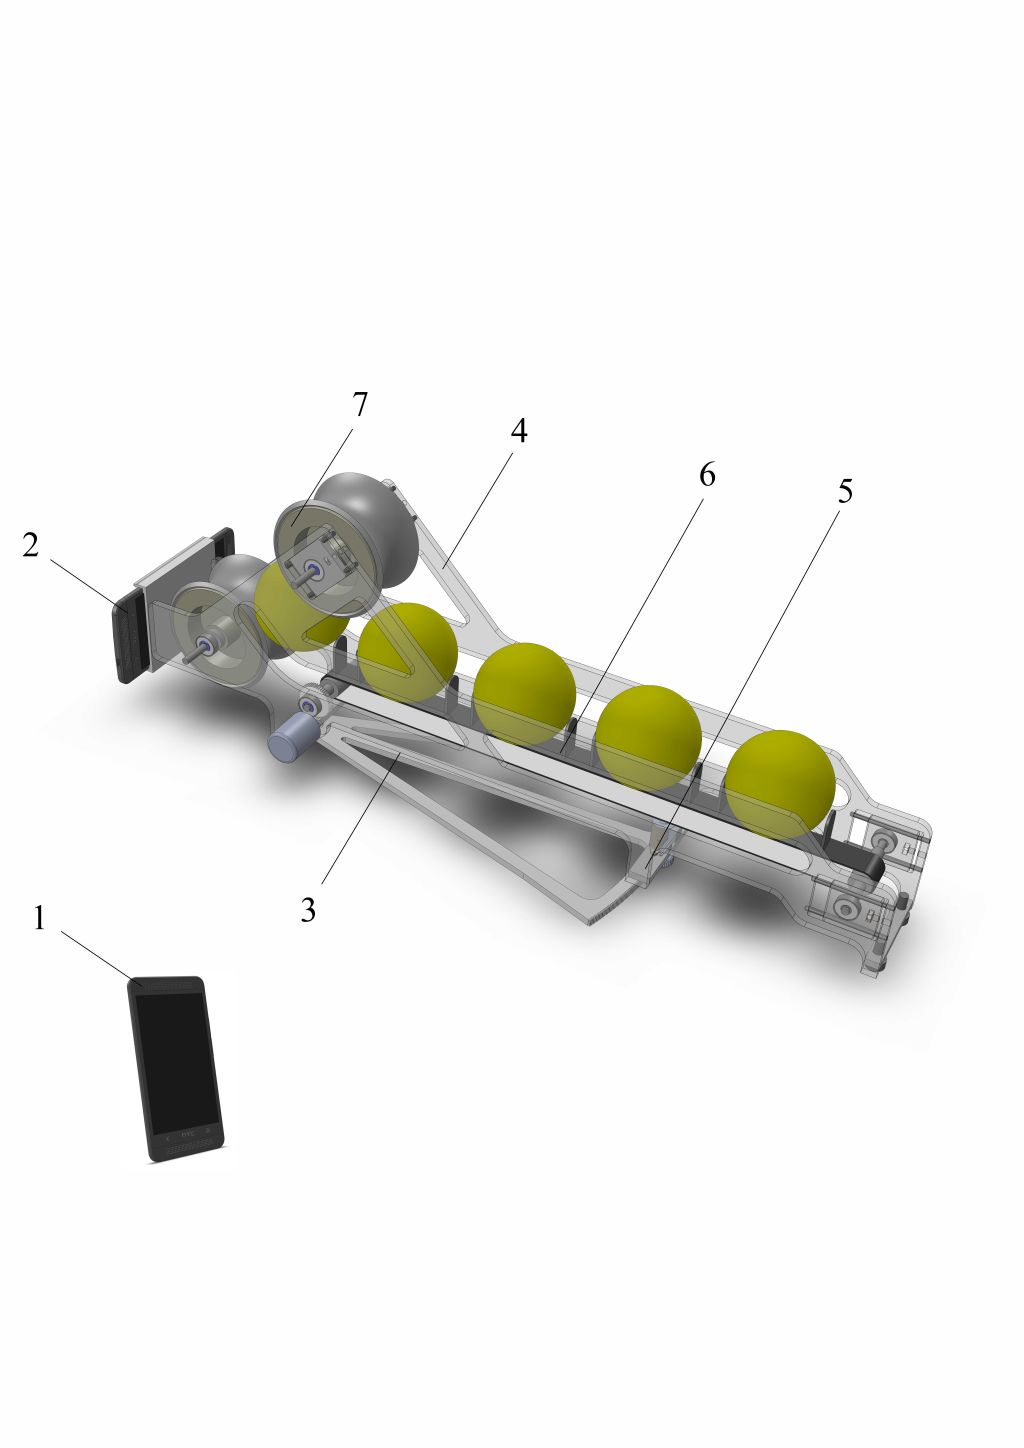
\includegraphics[width=0.95\textwidth,clip,trim=0mm 18mm 0mm 24mm]
		{Enddokumentation/Loesungskonzept/Bilder/Beschreibung_Komponenten-edited.jpg}
		\caption{Geräteübersicht}
		\label{fig:Geraeteuebersicht}
\end{figure}
\newpage
\begin{table}[h!]
	\begin{threeparttable} 
		\begin{tabular}{p{8mm}p{3.5cm}p{8.1cm}}
		    \textbf{Pos}\tnote{*} & \textbf{Bezeichnung} & \textbf{Funktion} \\ 
			\hline\rule{0pt}{11pt} 1 & Startgerät (Computer) & Senden des Startbefehls, Empfangen des Endbefehl, 
			Akustische und visuelle Signalausgabe \\ 
			    \rule{0pt}{11pt}   2 & Master  (Smartphone) & Empfangen des Startbefehls, Senden des Endbefehls,
			Fotografieren, Auswerten und Steuern des Controllers \\ 
			  \rule{0pt}{11pt}     3 & Controller & Steuerung und Regelung der Antriebe \\ 
			  \rule{0pt}{11pt}     4 & Gestell & Stabilisieren des Systems,	seitliche Führung der Bälle \\ 
			   \rule{0pt}{11pt}    5 & Horizontale\newline Ausrichteinheit & Ausrichten des Gerätes zum Korb \\ 
			   \rule{0pt}{11pt}    6 & Förderband & Ballförderung zu den Schwungräder \\ 
			   \rule{0pt}{11pt}    7 & Schwungräder & Beschleunigen der Bälle \\ 
		\end{tabular} 
		\centering
		\caption{Bezeichnung der Teilkomponenten}	
		\label{tab:BezTeilkomponenten}
		\begin{tablenotes}\footnotesize 
			\item[*] Die Position bezieht sich auf die Nummern in Abbildung \ref{fig:Geraeteuebersicht}.
		\end{tablenotes}
	\end{threeparttable} 
\end{table}
\parindent 0pt In den folgenden Abschnitten wird nach dem zeitlichen Ablauf des Balles, 
die einzelnen Komponenten des Ballwerfers näher beschrieben. 